\chapter{Introduction, Finite Automata, Regular Expressions}

The theory of computation begins with a question: What is a computer. The real computer is too complicated to understand, to start with, we use an idealized computer called \textbf{computational model}. 

The simplest model among them is \textbf{finite state machine} or \textbf{finite automaton}.  

\section{Finite Automata}

Finite automata are good models for computers with an extremely limited amount of memory. 

Finite automata and their probabilistic counterpart \textbf{Markov chains} are useful tools when we're attempting to recognize patterns in data. Markov chains have even been used to model and predict price changes in financial markets.

\begin{eg}[Finite Automata Example]
    Here's an example of finite automata:\\
    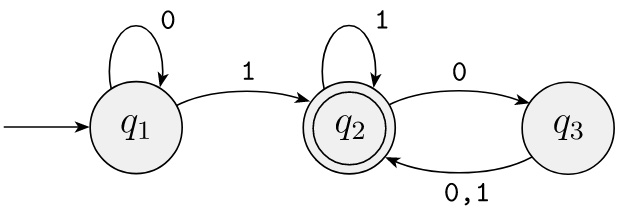
\includegraphics[width=\textwidth]{f1.4.jpg}

    \begin{itemize}
        \item The figure is called \textbf{state diagram} of \(M_1\).
        \item Three \textbf{states}: \(q_1\), \(q_2\) and \(q_3\).
        \item \textbf{Start state}: \(q_1\).   
        \item \textbf{Accept state}: \(q_2\).  
        \item The arrows going from one state to another are called \textbf{transitions}.
    \end{itemize}

    When the automaton receives an input string such as \verb|1101|, it processes that string and produces an output. The output is either \textbf{accept} or \textbf{reject}:
    \begin{enumerate}
        \item Start in state \(q_1\) 
        \item Read \verb|1|, follow transition from \(q_1\) to \(q_2\)  
        \item Read \verb|1|, follow transition from \(q_2\) to \(q_2\)  
        \item Read \verb|0|, follow transition from \(q_2\) to \(q_3\)  
        \item Read \verb|1|, follow transition from \(q_3\) to \(q_2\)  
        \item \(Accept\) because \(M_1\) is in an accept state \(q_2\) at the end of the input   
    \end{enumerate}
\end{eg}

\begin{definition}[Formal Definition of A Finite Automaton]
    A \textbf{finite automaton} is a 5-tuple (\(Q, \Sigma, \sigma, q_0, F\)), where
    \begin{enumerate}
        \item \(Q\) is a finite set called \textbf{state} 
        \item \(\Sigma\) is a finite set called the \textbf{alphabet} 
        \item \(\sigma: Q \times \Sigma \Rightarrow Q\) is the \textbf{transition function}
        \item \(q_0 \in Q\) is the \textbf{start state}
        \item \(F \subseteq Q\) is the \textbf{set of accept state}         
    \end{enumerate}
\end{definition}

\begin{eg}[Revisit Finite Automata Example]
    Let's revisit the finite automata example \(M_1\) and see from the formal definition perspective: \\
    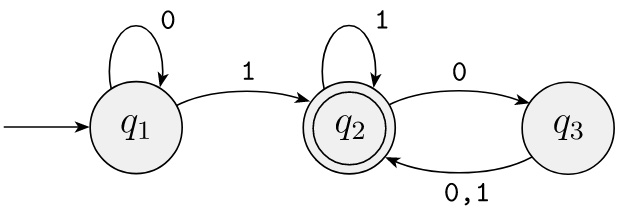
\includegraphics[width=\textwidth]{f1.4.jpg}

    We can describe \(M_1\) formally by writing \(M_1 = (Q, \Sigma, \sigma, q_1, F)\), where   
    \begin{enumerate}
        \item \(Q = \{q_1, q_2, q_3\}\)
        \item \(\Sigma = \{ 0, 1 \} \)  
        \item \(\sigma\) is described as 
        \begin{table}[H]
            \centering
            \begin{tabular}{c|c|c}
                \toprule
                     & 0 & 1  \\
                \midrule
                   \(q_1\)  & \(q_1\)  & \(q_2\)  \\
                   \(q_2\)  & \(q_3\)  & \(q_2\)  \\
                   \(q_3\)  & \(q_2\)  & \(q_2\)  \\
                \bottomrule
            \end{tabular}
        \end{table}
        \item \(q_1\) is the start state
        \item \(F = \{ q_2 \} \)  
    \end{enumerate}
\end{eg}

If A is the set of all strings that machine \(M\) accepts, we say that A is the \textbf{language of machine M} and write \(L(M) = A\).   
We say that \textbf{M recognizes A} or that \textbf{M accepts A}.     
Here because \(accept\) has different meaning, we use \(recognize\) for the language.  

\begin{remark}
    A machine may accept several strings, but it always recognizes only one language.
    If the machine accepts no strings, it still recognizes one language -- namely, the empty language \(\emptyset\). 
\end{remark}

\begin{eg}[Revisit Finite Automata Example: Language]
    In our example, the language set A can be represented as:

    A = \{\(\omega\)|\(\omega\) contains at least one \verb|1| and an even number of \verb|0|s follow the last \verb|1|\}.

    Then \(L(M_1) = A\), or equivalently, \(M_1\) recognizes \(A\).   
\end{eg}
